\section{Introduction}
As part of the ongoing study of the structure of nucleons \cite{Avakian:2010ae}  in Hall B at the Thomas Jefferson National Accelerator Facility (JLab), the CEBAF Large Acceptance Spectrometer (CLAS12) \cite{Burkert:2020akg} is being used to accurately identify the secondary particles of high energy reactions, to assist in probing the strangeness frontier, and to aid in characterizing the transverse momentum distribution (TMD) and generalized parton distribution (GPD) functions of the nucleon. Indispensable to this task is the ability to identify kaons, pions, and protons.  With the CLAS12 spectrometer providing accurate momentum measurements, the Ring Imaging Cherenkov detector (RICH) \cite{Contalbrigo:2020,Contalbrigo:2020snw,Mirazita:2017vav,Contalbrigo:2014rqa} provides tandem Cherenkov light-cone radius measurements that yield the velocities of near light-speed particles, thus facilitating mass-dependent particle identification.

\begin{figure}[h!bt]
	\centering
	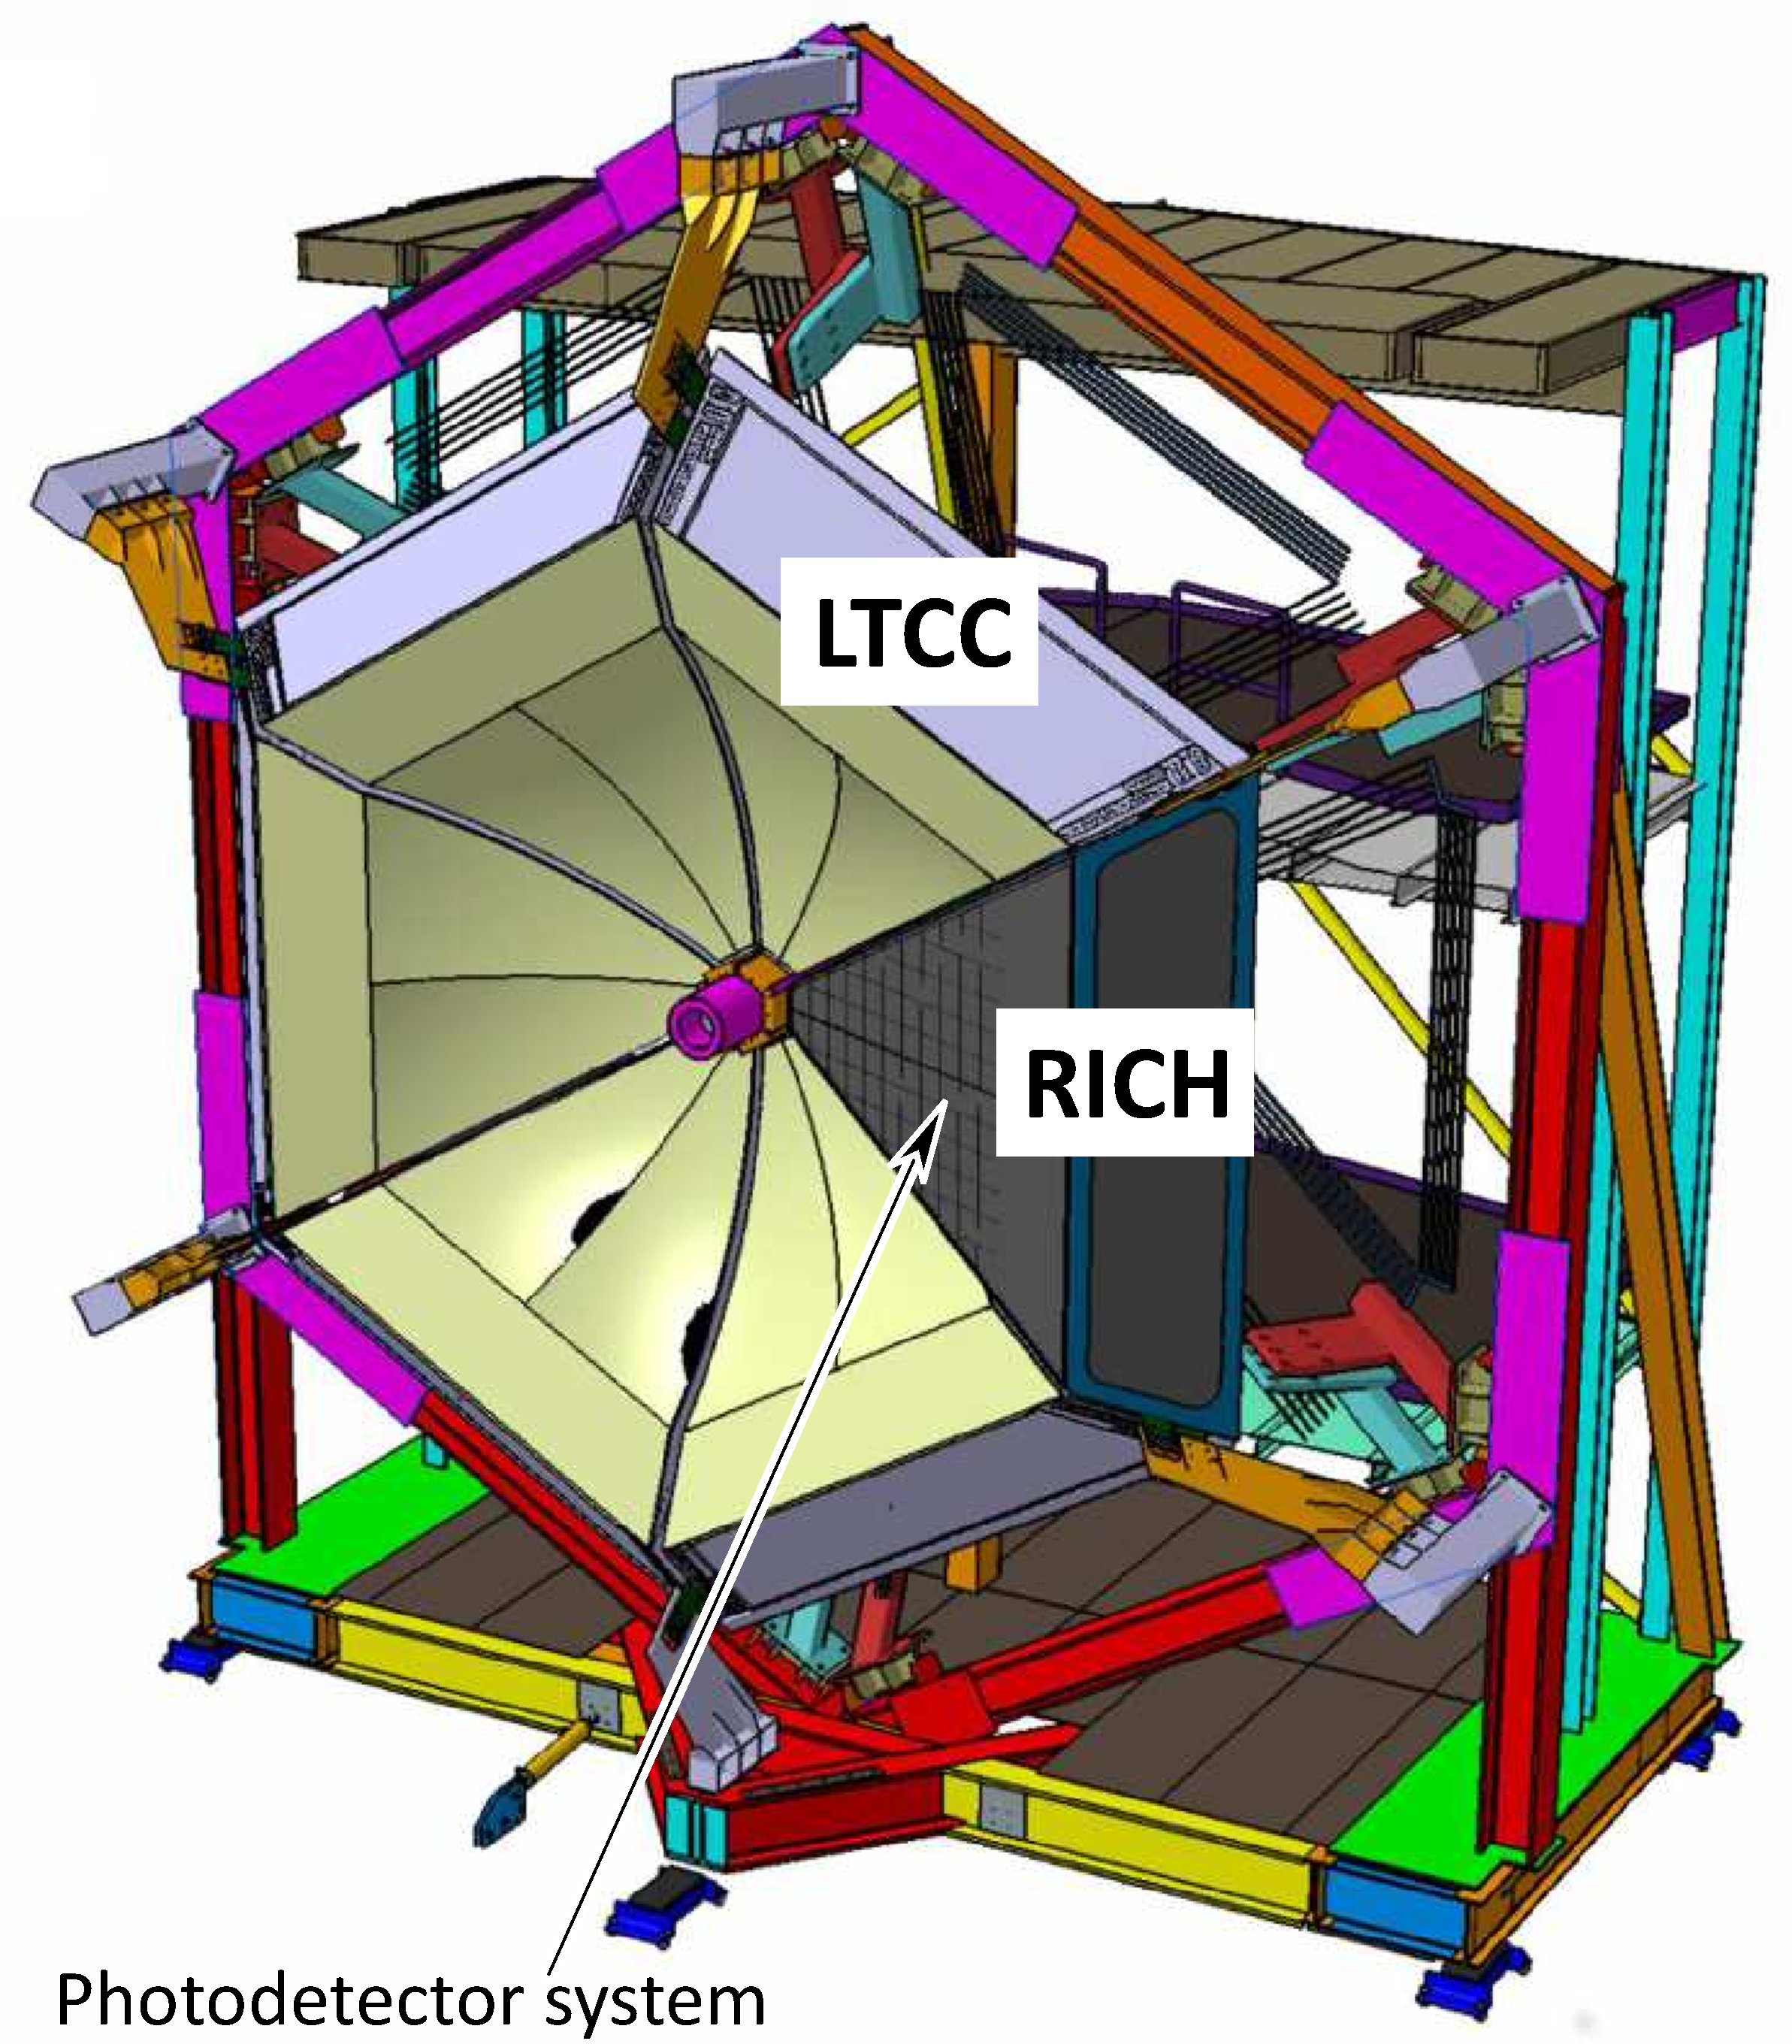
\includegraphics[width=0.95\linewidth]{figures/RICHdetector.pdf}
	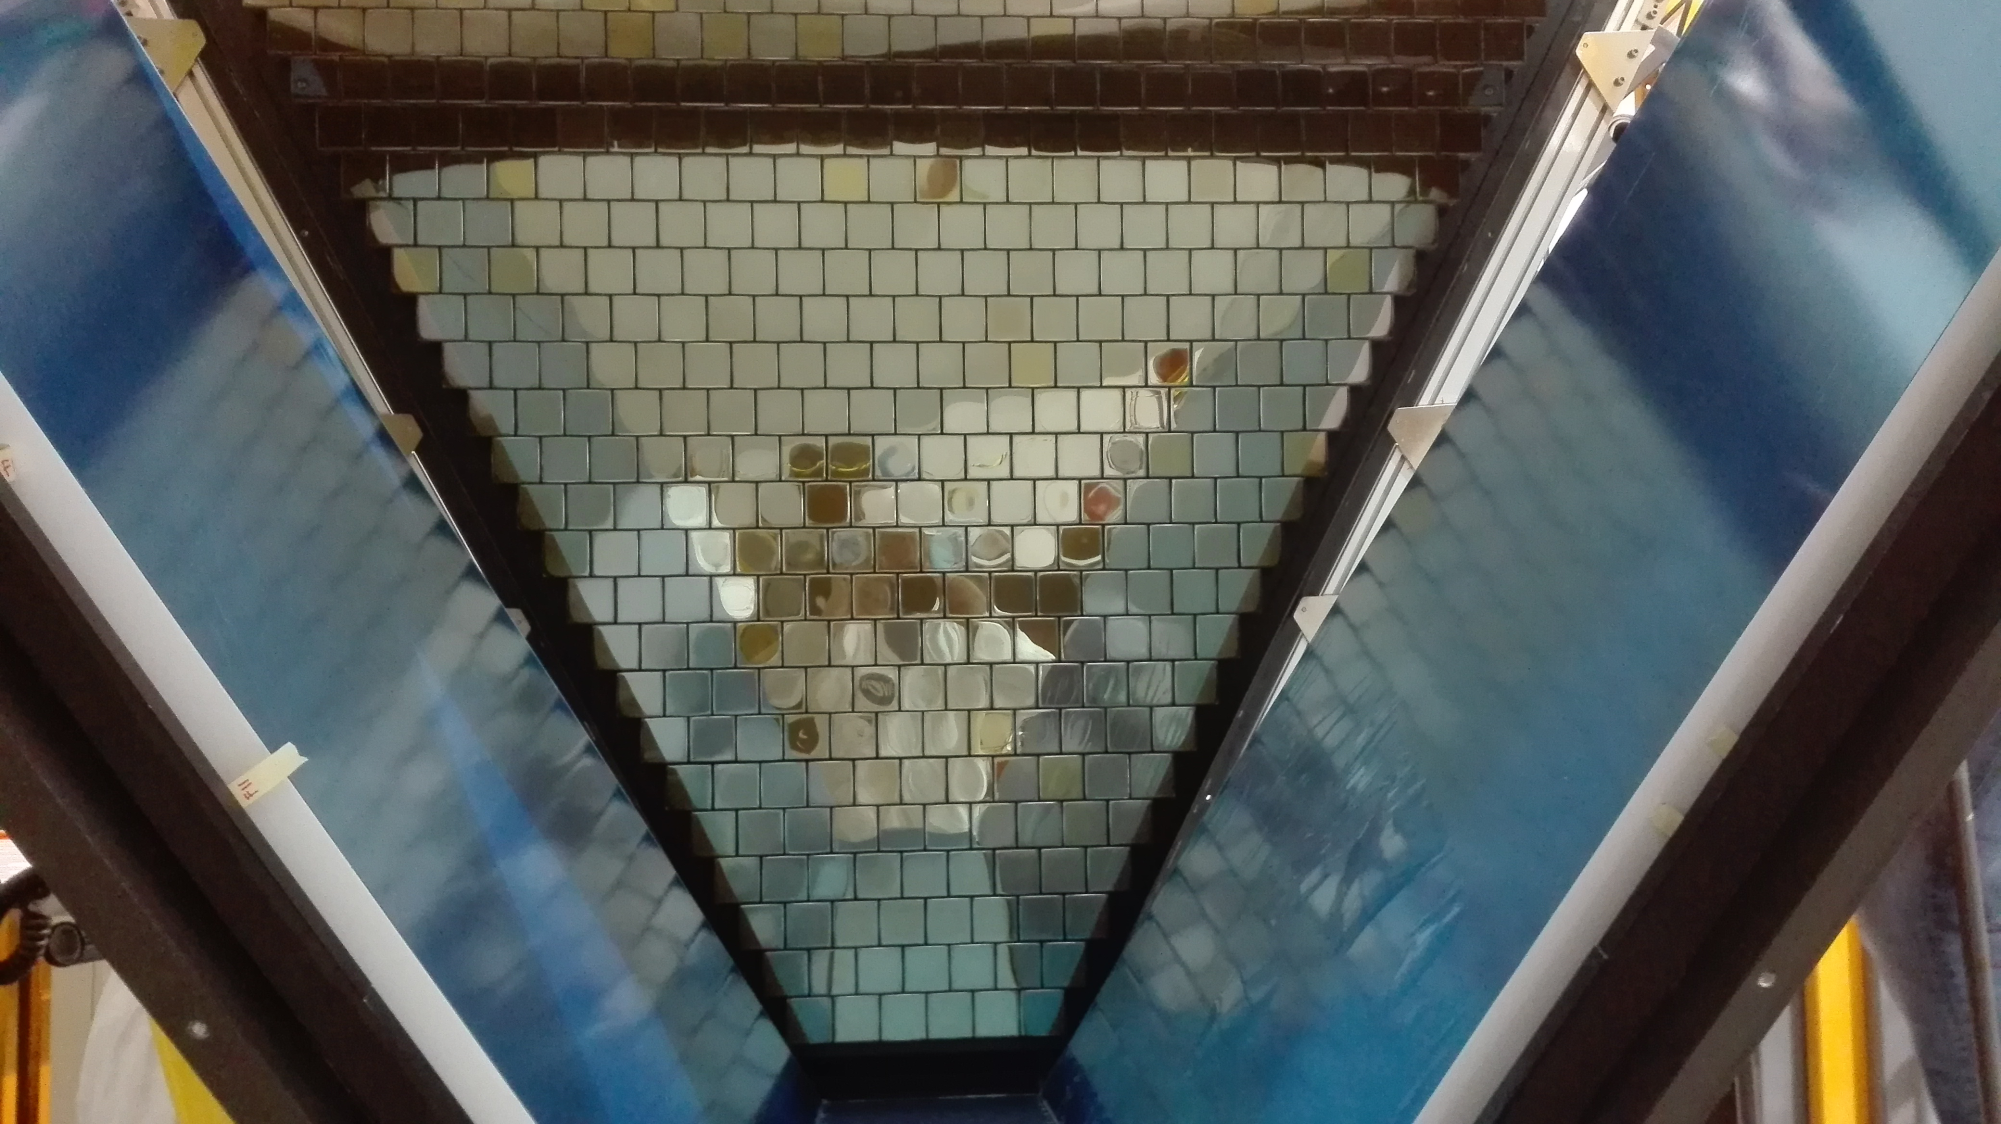
\includegraphics[width=0.95\linewidth]{figures/RICHpanel_front.png}
	\caption{Top: The part of the CLAS12 detector with the RICH covering one out of six sectors. Bottom: the photomatrix of multianode photomultipliers and the mirror system.}
	\label{fig:RICHdetector}
\end{figure}

The photomatrix  wall is a crucial component of the RICH detector (see Fig.~\ref{fig:RICHdetector}). It is relatively large (area about 1 m$^2$) and should be comprised of many photon detection devices such as photomultiplier tubes.
Due to the imaging aspect of the RICH they must provide a spatial resolution of less than 1 cm.
Since multiple photon detectors are tiled into large arrays, they should have large active area with minimal dead-space.
The photon detectors must also efficiently detect single photon level signals and should be sensitive to visible light due to the aerogel radiator material.
Multianode Photomultiplier Tubes from Hamamatsu are perfect candidates for the CLAS12 RICH detector, as they are flat-panel PMTs offering an adequate compromise between detector performance and cost.
Each MaPMT consists of an 8 by 8 array of pixels, each with dimension of 6~mm x 6~mm.
Furthermore, the device has a very high packing fraction of 89\% with a high quantum efficiency of 20-30\% in the visible light region.
The tubes also have excellent immunity to magnetic fields because all internal parts are housed in a metal package and the distance between dynode electrodes is very short.


Initially, the Hamamatsu H8500 MaPMT model \cite{H8500} was chosen as the best option because they provide high quantum efficiency for visible light and sufficient spatial resolution (6x6 mm$^2$) at a limited cost.
However, Hamamatsu has released the new H12700 MaPMT model  \cite{H12700} that shows enhanced single photoelectron (SPE) detection, reduced crosstalk between pixels, and is otherwise similar in spatial resolution and  cost to the H8500 MaPMTs.
The first RICH detector was installed in sector 4 of the CLAS12 detector in 2018.
There are 391 Hamamatsu MaPMTs  in the photodector matrix, 76 of them are H8500 and 315 H12700. 
The second RICH detector is almost identical to the first one and presently under construction scheduled to be installed soon.
%The initial characterization of these PMTs was done using a laser stand equipped with a crate of Flash ADC  boards \cite{FADC250} because the custom RICH front-end electronics \cite{RICH_FE} was not ready at that time.
The characterization of MaPMTs for both detectors was done using a laser stand equipped with custom front-end electronics boards which have much better parameters than the FADCs~\cite{FADC250} used for preliminary studies and installed in the most of the CLAS12 subsystems.
This highly integrated front-end (FE) electronics with modular design~\cite{RICH_FE} was developed for a large array of Hamamatsu H8500 and H12700 MaPMTs to minimize the impact of the electronics material on the CLAS12 subsystems downstream of the RICH detector.
The architecture of the readout electronics consists of front-end cards with dedicated Application Specific Integrated Circuits (ASICs), configured, controlled, and read out by Field Programmable Gate Arrays (FPGAs) \cite{RICH_FE}.
The ASIC board is based on the MAROC3  integrated circuit \cite{MAROC} whose excellent single photon capabilities both in analog and binary mode have been confirmed.
%The final design has consists of stacked PCB layers behind each MaPMT sensor (see~Fig.~\ref{fig:feboards}).
%The first layer houses the ASIC front end and ancillary components (e.g. external amplifier) and it is directly connected to the anodes array.
%A second PCB will host the FPGA in charge of configuring, managing and acquiring one or more ASICs and the low voltage and HV bias distribution.
%The use of the JLab SSP as controller and collector of the front-end data provides a strong synergy with the current JLab upgrade activity.
%Data are transmitted on high speed serial (optical) lines minimizing the wiring and therefore the material budget.
%With that sandwich architecture the total photon detection surface will be covered by a fixed number of basic units or tiles made up by two or three sensor each.
%The total spacing for electronics will not exceed 20 cm in depth (including MaPMT and mechanical support).
The three-tile electronics module with and without the three H12700 MaPMTs installed is shown in~Fig.~\ref{fig:feboards}.
The performance of the MAROC chips was tested and was found suitable for the RICH requirements:
\begin{itemize}
	\item 100\% efficiency at 1/3 of the single photoelectron signal (50~fC)
	\item time resolution of 1~ns
	\item short deadtime to sustain a trigger rate of 30~kHz
	\item latency of 8~$\mu$s
\end{itemize}
We made detailed characterization of around 400 H12700 MaPMTs, as well as several H8500 to make a comparison of the two models. These data turned out to be useful for evaluating the performance of the first CLAS12 RICH detector where both MaPMT models are used. The single photoelectron spectra were measured for each pixel at different high voltages and light intensities of the laser test setup. Using the dedicated front-end electronics, standard for the RICH detectors, the setup allowed us to characterize each pixel’s properties such as gain, quantum efficiency, signal crosstalk between neighboring pixels, and determine the signal threshold values to optimize their efficiency to detect Cherenkov photons. These parameters were determined for each pixel in the set of 400 MaPMTs, giving us the opportunity to select the best MaPMTs and determine the working parameters of the front-end electronics in the real experiment. The results of this study are presented in this paper. 
%These data turned out to be useful for evaluating the first RICH performance  where we are using both MaPMT models. The single photoelectron spectra were measured for each pixel at different high voltages and light intensities of the laser test setup. Using the standard for RICH dedicated front-end electronics the setup allowed us to characterize each pixel’s properties such as gain, quantum efficiency, signal crosstalk between neighboring pixels, and determine the signal threshold values to optimize their efficiency to detect Cherenkov photons. These parameters were determined for each pixel out of 400 MaPMTs what gives us the possibility to select the best MaPMTs and determine the working parameters of the front-end electronic in the real experiment. The results of this study are presented in this paper. 


The remaining structure of this paper is laid out as follows. 
\begin{itemize}
	\item Section 2 presents the design of the laser test stand for the MaPMT automated characterization, allowing illumination of every pixel by the precisely calibrated low light pulses in the controlled stable environment, and collecting the response data. 
	\item Section 3 describes the procedures for the absolute calibration of the readout electronics converting the output signal amplitudes to linear charge scale in pC for every pixel. 
	\item Section 4 illustrates the techniques for the pixel-to-pixel crosstalk measurements, and possible algorithms for the separation of the crosstalk from real signals. 
	\item Section 5 describes the technique of absolute calibration of the light source, as a prerequisite for the measurement of quantum efficiency in every pixel. 
	\item Section 6 describes the computational model used in the data analysis to extract such critical parameters for each anode, as its quantum efficiency, gain, the shape of the single photoelectron amplitude response function, and contribution of the crosstalk signals from the neighboring pixels, and introducing the novel technique of characterizing the crosstalk contributions in the model. 
	\item Section 7 illustrates the self-consistency of the algorithm for the parameters' extraction using the measurements at different light intensities and different high voltages applied. 
	\item Section 8 presents the results of the full characterization and study of all 399 MaPMTs, showing the spread of the extracted parameters and evaluating the systematic errors from the independent redundant measurements. The results make possible the evaluation of average and individual pixel characteristics of the full MaPMT array for the purposes of selection and arrangement of the MaPMTs in the RICH detector, and for use in the experimental data analysis.
\end{itemize}

\begin{figure}[htb]
  \centering
  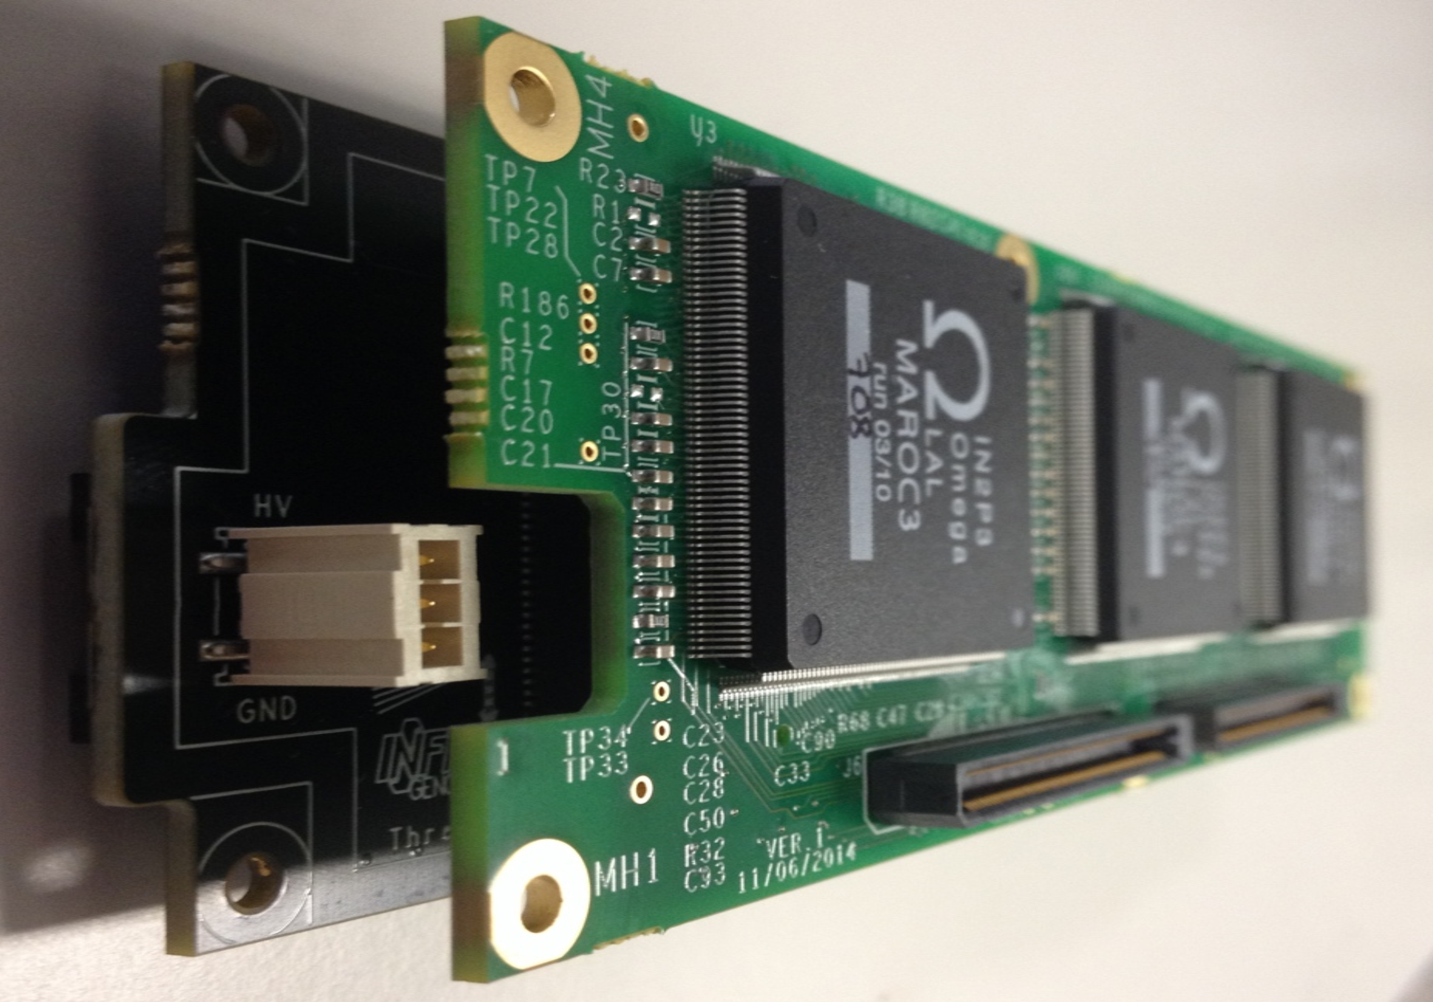
\includegraphics[width=0.8\linewidth]{figures/fe1.pdf}
  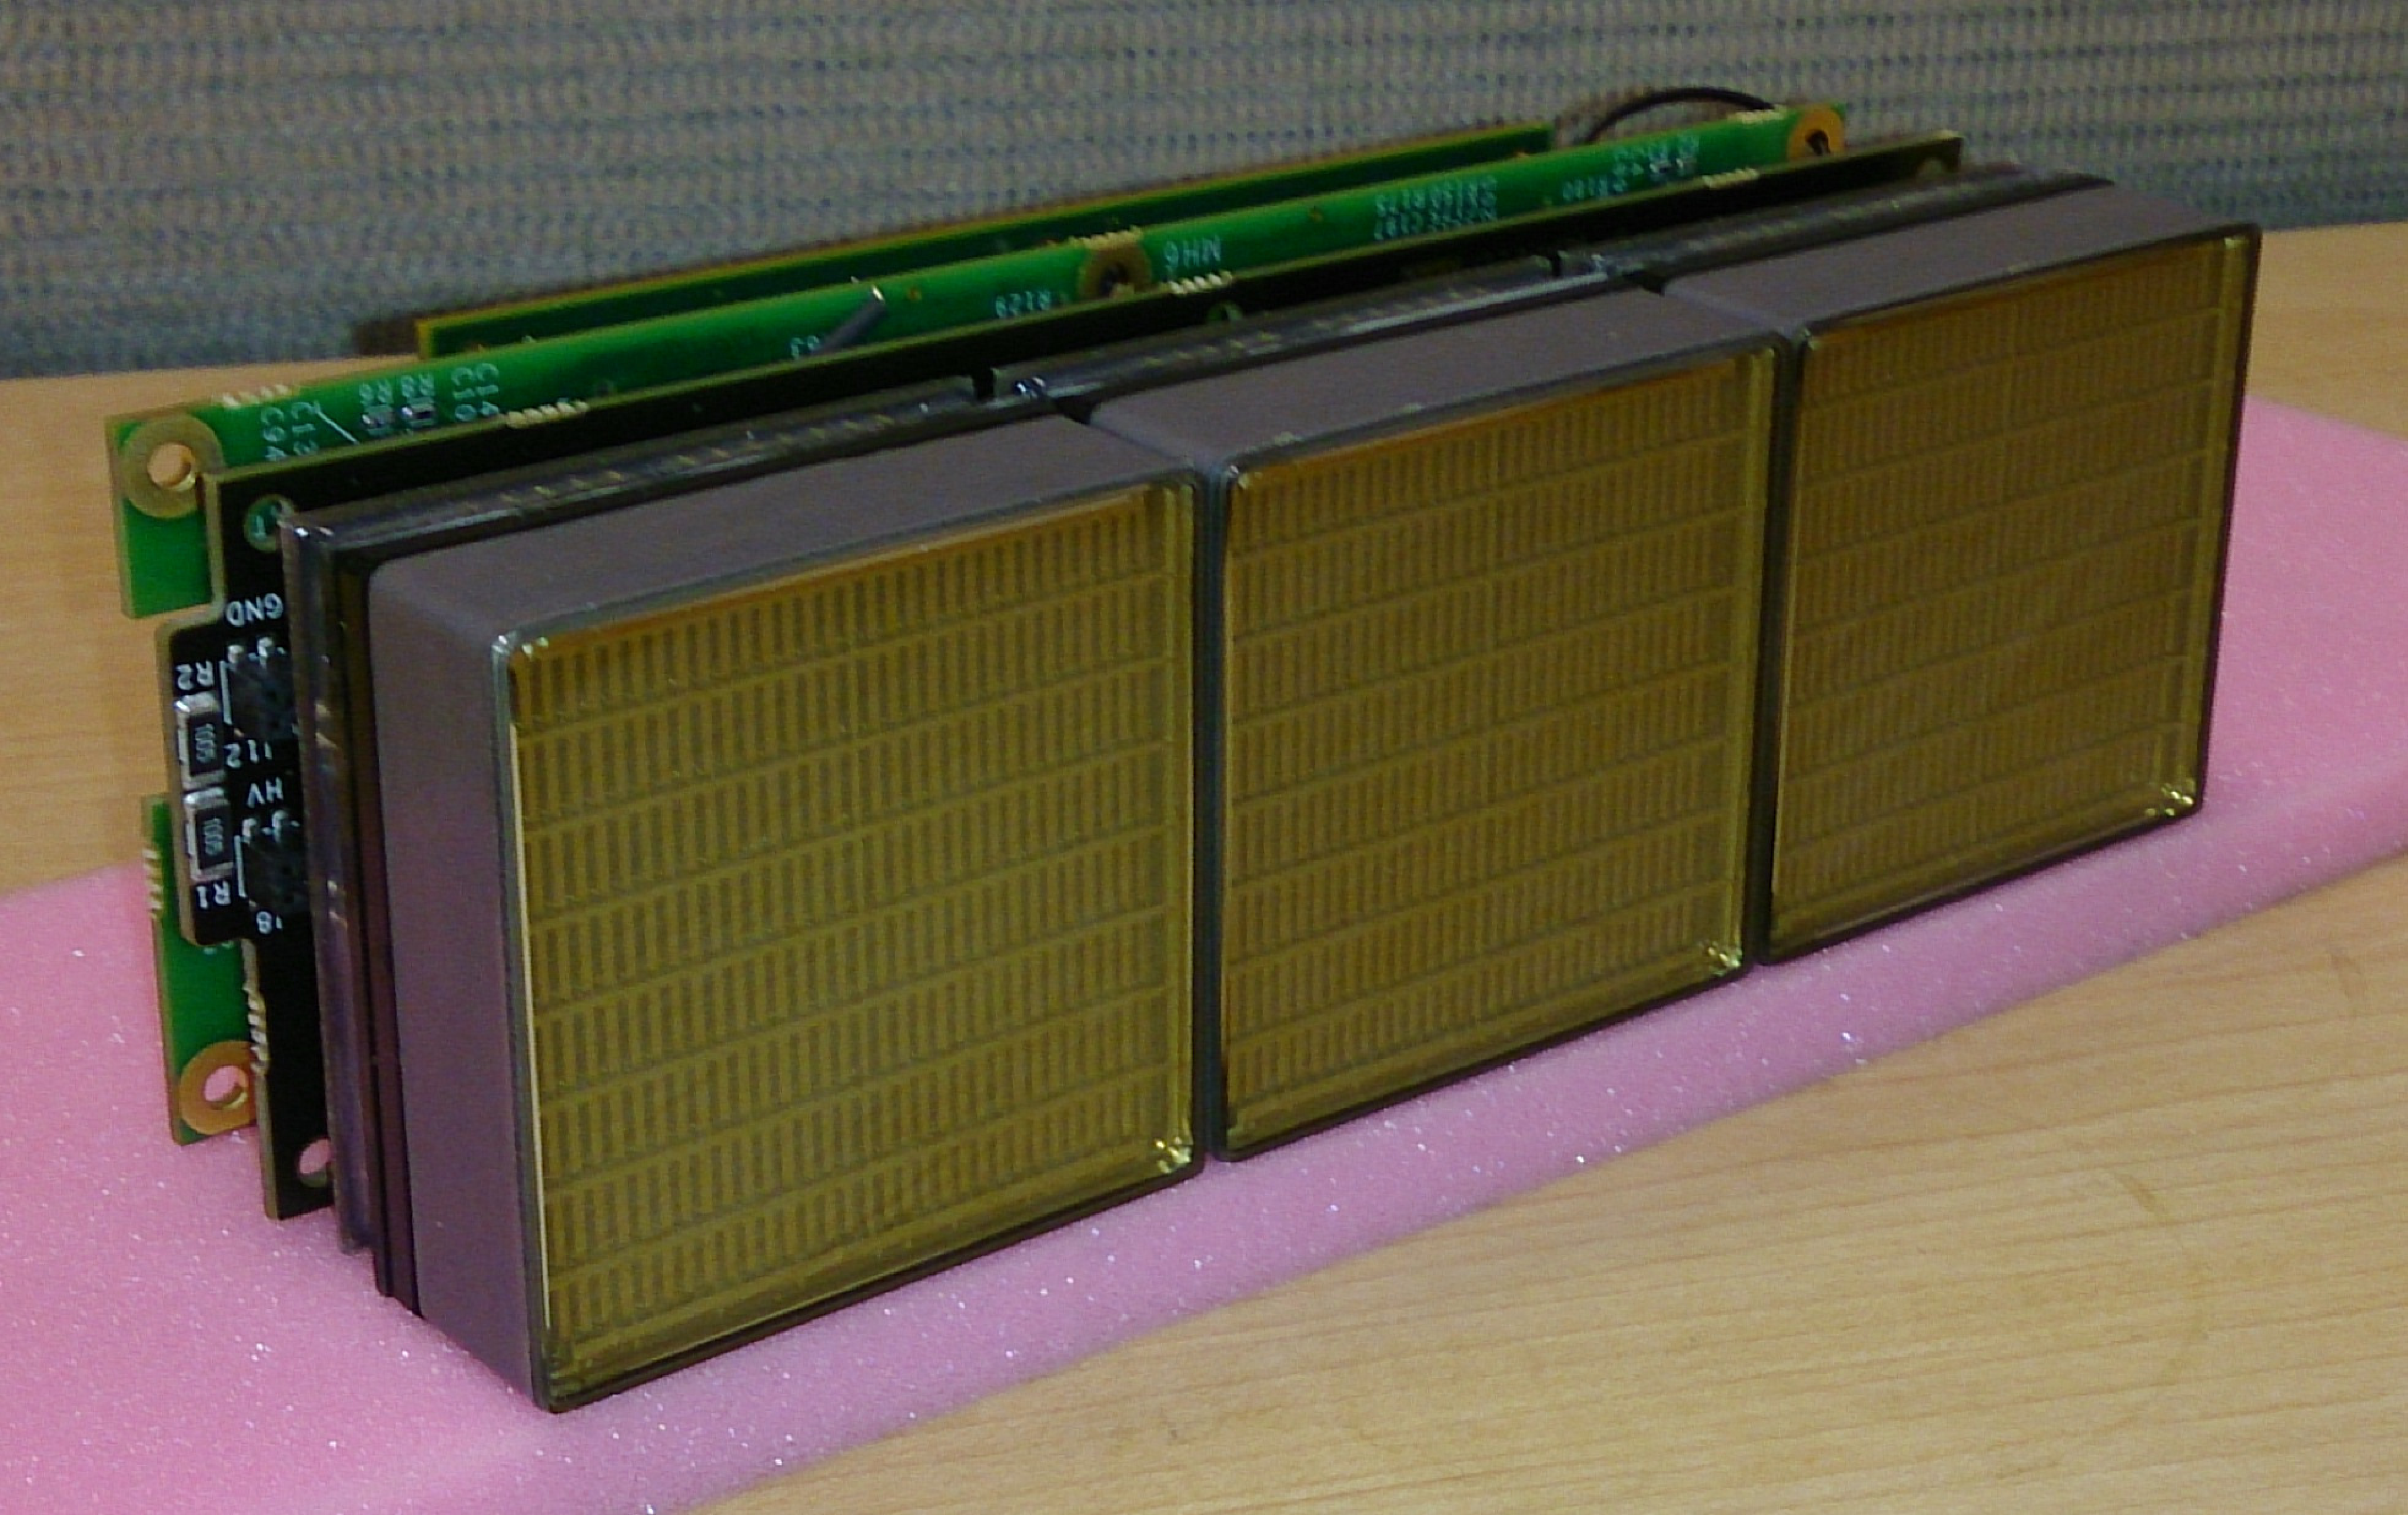
\includegraphics[width=0.8\linewidth]{figures/frontendPMT.pdf}
  \caption{Front-end electronics readout board and mounted MaPMTs.}
  \label{fig:feboards}
\end{figure}






